\documentclass[english]{article}
\usepackage{graphicx}
\usepackage{amsmath}
\usepackage{hyperref}
\usepackage{setspace}
\usepackage{apacite}
\usepackage{hyperref}
\usepackage{natbib}
\usepackage{pxfonts}
\usepackage[utf8]{inputenc}
\usepackage[left=1in,right=1in,top=1in,bottom=1in]{geometry}
\usepackage[left]{lineno}
\usepackage{soul}
\usepackage[table]{xcolor}
\usepackage{colortbl}
\usepackage{booktabs}
\usepackage{longtable}
\usepackage{lscape}
\usepackage{rotating}
\usepackage{supertabular}

\linenumbers

\newcommand{\synth}{1}
\renewcommand{\thefigure}{S\arabic{figure}}
\renewcommand{\thetable}{S\arabic{table}}

\title{\textit{Supplemental materials for:} High-order cognition is supported by information-rich but compressible brain activity patterns} 

\author{Lucy L. W. Owen\textsuperscript{1, 2} and Jeremy R. Manning\textsuperscript{1,
*}\\\textsuperscript{1}Department of Psychological and Brain Sciences,\\Dartmouth College,
Hanover, NH\\[0.1cm]\textsuperscript{2}Carney Institute for Brain Sciences,\\Brown University,
Providence, RI\\[0.1cm] \textsuperscript{*}Address correspondence to
jeremy.r.manning@dartmouth.edu}

\begin{document}
\maketitle


% \begin{figure}
%   \centering
%   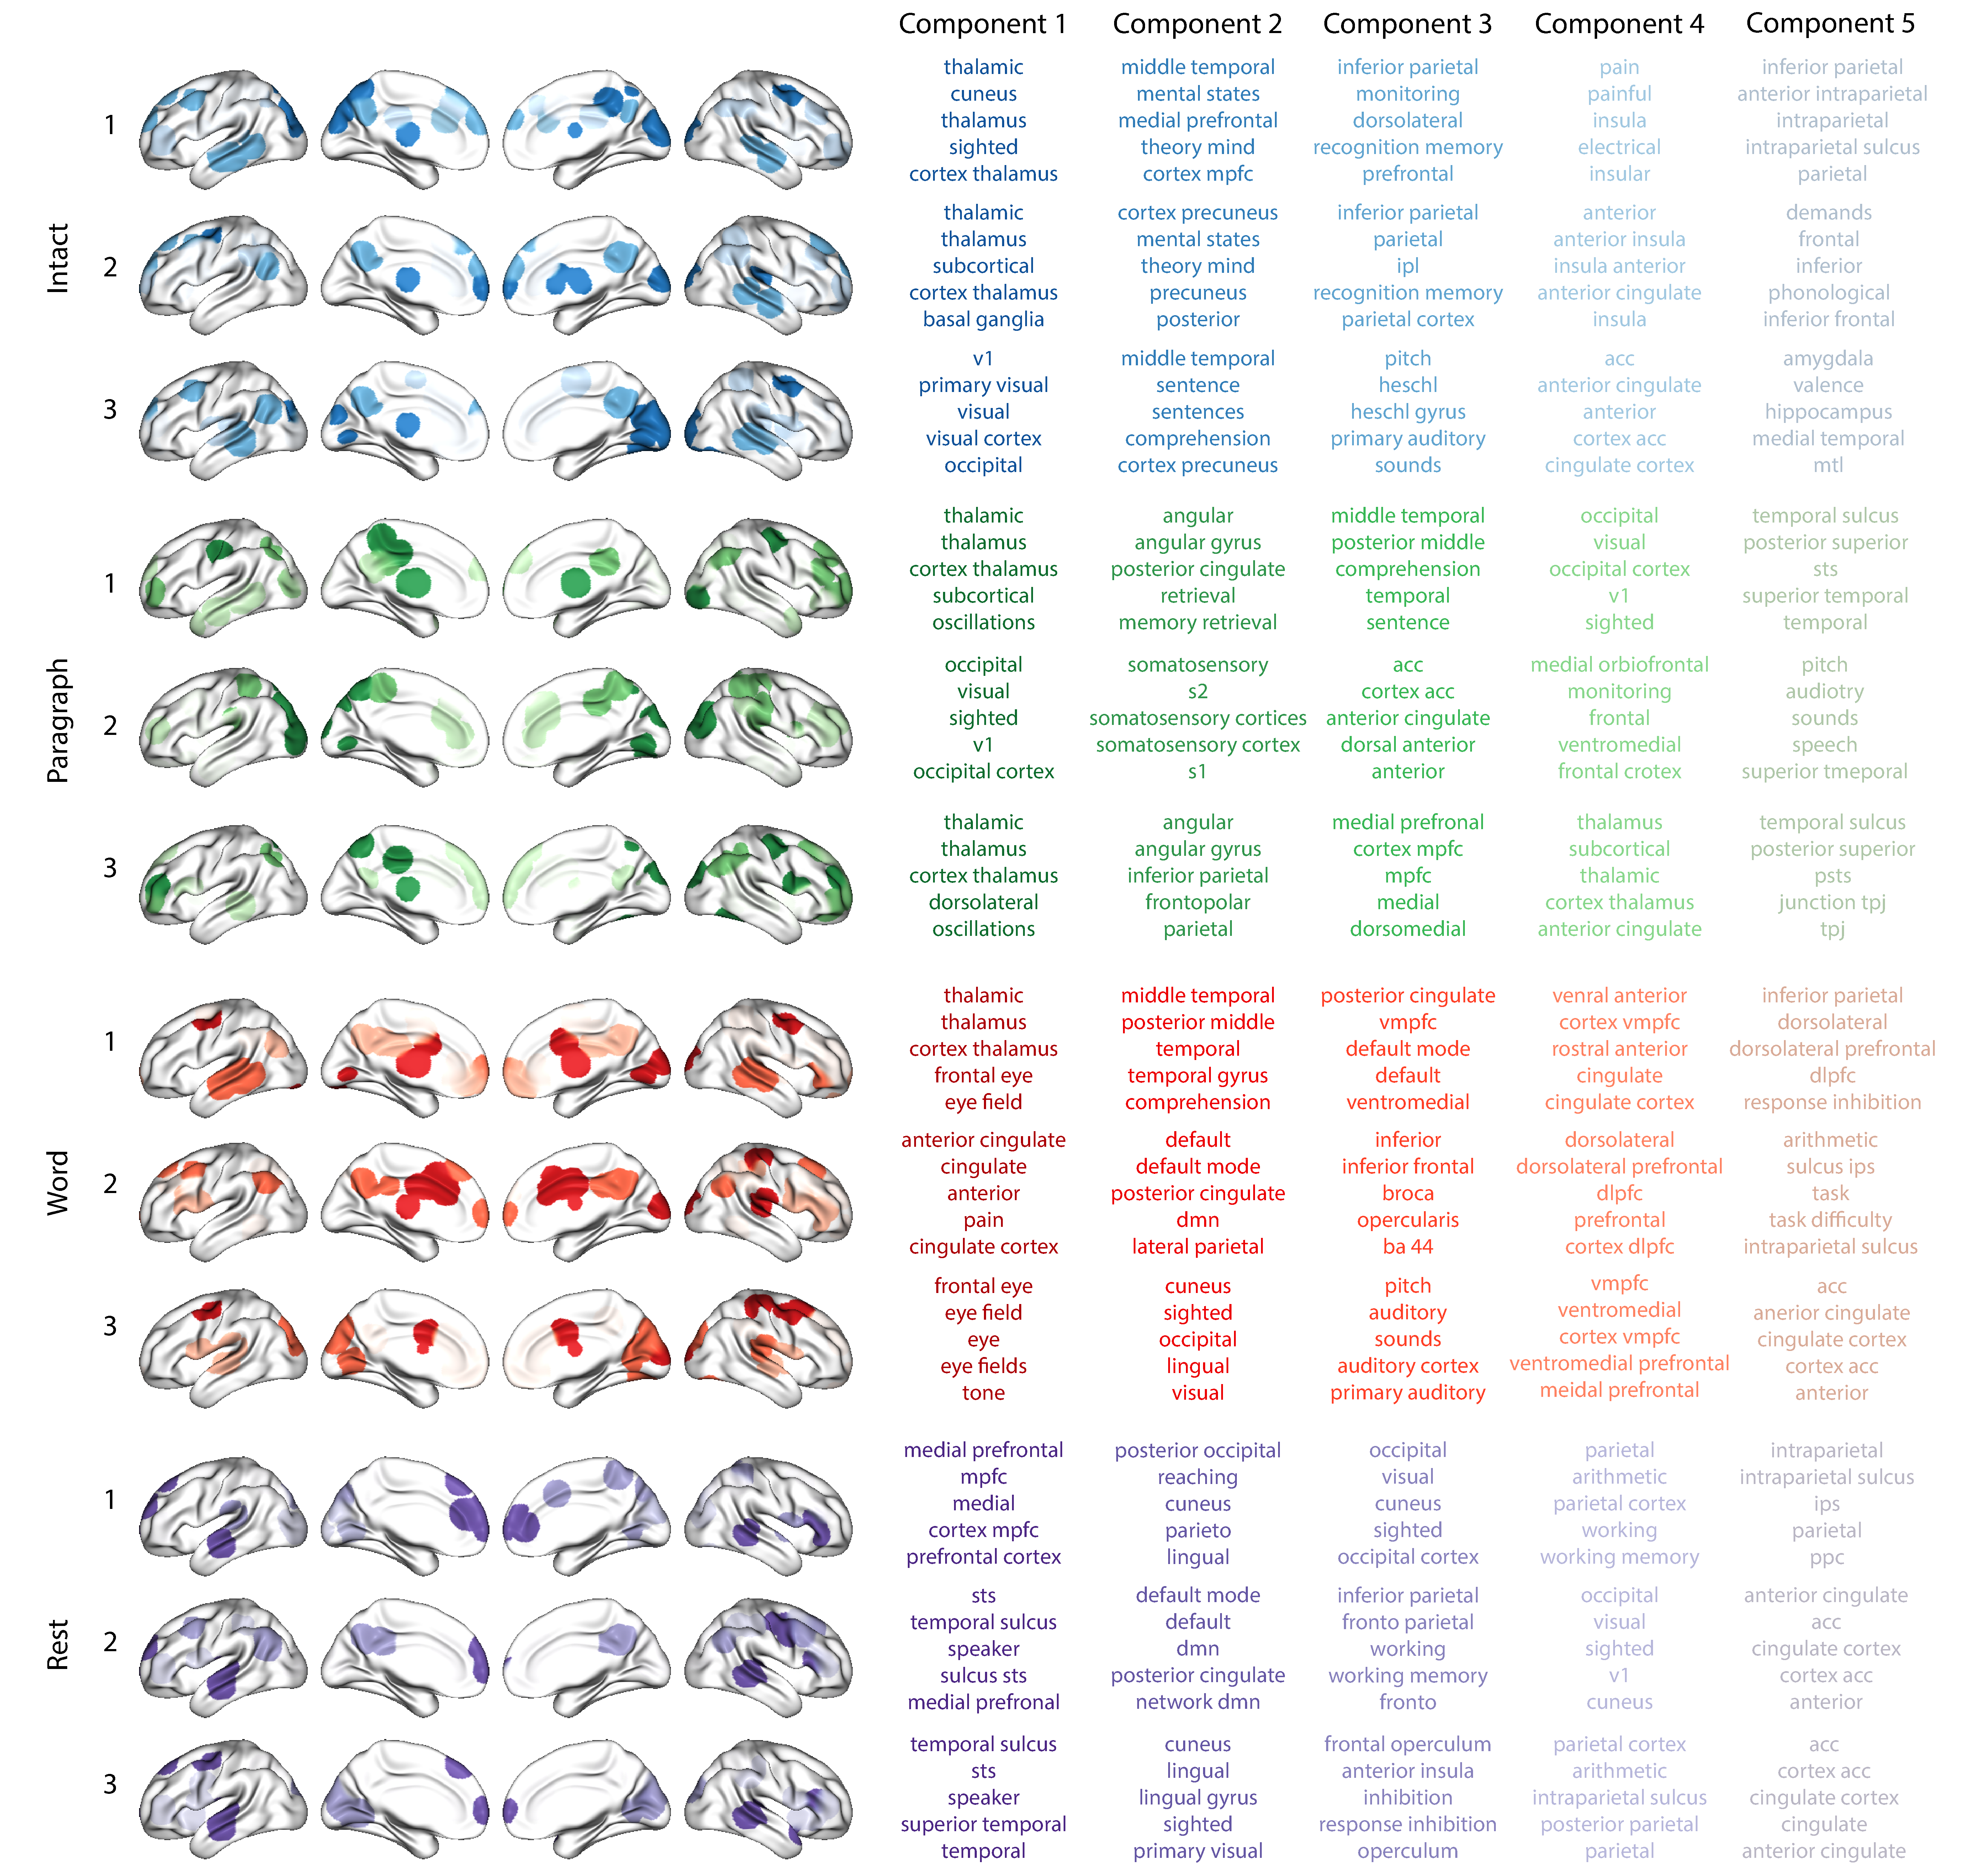
\includegraphics[width=\textwidth]{figs/pca_neurosynth_thirds}

% \caption{\textbf{Top terms associated with the highest-weighted components by
% condition, broken down by story segment.} Each group of three rows corresponds
% to an experimental condition, and the colors correspond to the component number
% (ranked by proportion of variance explained). The rows' numbering denotes the
% story segment used to compute each map (1: first third; 2: second third; 3:
% third third). The inflated brain plots display the top 20 highest-weighted hubs
% (see \textit{Topographic Factor Analysis}) for each components. The lists on
% the right display the top five Neurosynth terms~\citep{RubiEtal17} decoded from
% each components' brain map. Analogous maps computed for the entire story may be
% found in Figure~\synth.}

% \label{fig:neurosynth-thirds}

% \end{figure}

\begin{landscape}
  \tablehead{\toprule
  Topic label &     Cognitive label &           Term 1 &        Term 2 &          Term 3 &         Term 4 &      Term 5 &         Term 6 &        Term 7 &         Term 8 &        Term 9 &        Term 10 \\
  \midrule
  }
  \tabletail{\bottomrule}
  \tiny

\begin{supertabular}{rlllllllllll}
  Cognitive control and task performance &   Cognitive control &            tasks &       control &         network &     conditions &  comparison &      performed &        common &     correlates &    experiment &            pre \\
  Developmental aging and maturation &                   - &              age &        adults &        children &    development & adolescents &          aging & developmental &    adolescence &     childhood &          adult \\
  Eye movements and visual attention &           Attention &              eye &          gaze &            eyes &         visual &    saccades &      movements &       saccade &      direction &          gait &         target \\
        Facial and voice recognition &  Sensory perception &      recognition &      familiar &        identity &     unfamiliar &       voice &    familiarity &         route &         voices &            fg &         facial \\
Social interaction and contextual behavior &    Social cognition &          context &          game &           human &    interaction &         ppi &     contextual &      contexts &         agency &  interactions &        partner \\
Language processing and semantic knowledge & Language processing &         semantic &         words &            word &        lexical &      verbal &       language &         tasks &         naming &       fluency &   phonological \\
Experimental design and behavioral performance &                   - &           trials &      stimulus &       responses &          trial &    reaction &           time &         event &         target &        events &          times \\
Genetic polymorphisms and risk factors &                   - &         carriers &        allele &            gene &       genotype &         met &        genetic &  polymorphism &            val &          comt &             rs \\
Sensorimotor integration and movement control &       Motor control &            motor &      movement &       movements &   sensorimotor &     primary &         finger &       control &        imagery &       sensory &      execution \\
  Drug addiction and substance abuse &                   - &          cocaine &         users &            drug &            bpd &    controls &       cannabis &     addiction &        craving &     dependent &         heroin \\
Music perception and auditory processing &  Sensory perception &            music &       musical &           pitch &       auditory &   musicians &      sequences &        rhythm &      listening &          beat &        singing \\
Menstrual cycle and hormonal regulation &                   - &            phase &         women &           cycle &         phases &   menstrual &             hf &    expression &            sex &        luteal &     follicular \\
Cognitive functions and role playing &   Cognitive control &             role &          play &           human &          plays &   cognitive &       evidence &      critical &       distinct &           key &     subregions \\
   Inhibition and gender differences &                   - &       inhibition &         women &      inhibitory &            sex &     females &         gender &         males &           stop &          male &         female \\
Somatosensory stimulation and motor control &       Motor control &      stimulation & somatosensory &             tms &        tactile &     primary &          touch &         motor &           rtms &  transcranial &        sensory \\
Multisensory integration and perception &  Sensory perception &         auditory &        visual &         sensory &       modality &      sounds &    integration &         sound &       stimulus &       primary &     modalities \\
       Social perception and empathy &    Social cognition &           social &       empathy &      experience &         people &      person &      responses &   perspective &    individuals &    attachment &       empathic \\
Gesture recognition and visual attention &           Attention &           target &      gestures &         targets &    orientation &      visual &    distractors &       gesture &          grasp &    distractor &       location \\
                 Experimental design &                   - &           design &         block &          blocks &          event &       mixed &      condition &            ca &        writing &       blocked &           runs \\
              Alcohol cue reactivity &              Reward &             cues &           cue &         alcohol &   anticipation &        cued &    preparation &  anticipatory &       exposure &    expectancy &    preparatory \\
         Neuroimaging and metabolism &                   - &              pet &    tomography &        emission &       positron &        flow &        glucose &       binding &     metabolism &     metabolic &       receptor \\
      Abnormalities in schizophrenia &                   - &    schizophrenia &      controls &         reduced &  abnormalities &    symptoms &       deficits &       matched &        control &      abnormal &  schizophrenic \\
              Eating and body weight &                   - &             food &         taste &            body &         weight &      eating &          women &         obese &         reward &         foods &        caloric \\
      Sleep and olfactory processing &  Sensory perception &            sleep &     olfactory &            odor &             sd & deprivation &          odors &           rem &    wakefulness &         night &           wake \\
Alzheimer's disease and mild cognitive impairment &                   - &               ad &       disease &             mci &      alzheimer &   cognitive &     impairment &          mild &           amci &      controls &        atrophy \\
Working memory and executive function &              Memory &           memory &          load &           tasks &         verbal & maintenance &    performance &          term &     difficulty &          dual &      cognitive \\
   Moral decision making and phobias &                   - &            moral &        phobia &          phobic &             ec &       guilt &         spider &      decision &            art &       phobics &    intentional \\
                 Language laterality & Language processing &         language &     asymmetry &    organization &          human &   dominance &    asymmetries &   lateralized &         handed &       located & representation \\
                           Attention &           Attention &        attention &   attentional &          visual &        spatial &         top &      selective &      stimulus &        control &     orienting &         target \\
Resting-state brain activity in smokers &       Resting state &             reho &       smokers &         resting &        smoking &    nicotine &    homogeneity &           sci &       controls &            rs &    spontaneous \\
           Social cognition/judgment &    Social cognition &           social &     judgments &            mind &         mental &      theory &    mentalizing &     cognition &       judgment &        person &         people \\
          Reward and decision making &              Reward &           reward &      decision &          choice &       outcomes &     rewards &       monetary &     decisions &   anticipation &     responses &        outcome \\
         ADHD and attention deficits &           Attention &             adhd &      disorder &       attention &        deficit &    children &  hyperactivity &      deficits &        control &      controls &        reduced \\
Neurobiological variability and individual diff... &                   - &       individual &  relationship &           local &      dependent &      change &         global &     responses &       neuronal &     magnitude &          lower \\
                   Spatial cognition &   Spatial cognition &          spatial &         space &        location &      locations &  navigation &        virtual &        visual &   visuospatial &         visuo &       position \\
Therapeutic interventions and training &                   - &         training &   acupuncture &         therapy &             cr &     control &        trained &   improvement &    mindfulness &   stimulation &        induced \\
      Color perception and deception &  Sensory perception &            color &        search &         feature &      deception &    features &      responses &        colour &      dimension &         lying &    conjunction \\
Neurodegenerative diseases and disorders &                   - &          disease &            pd &        controls &        atrophy &    clinical &          motor &      dementia &             sd &      multiple &      sclerosis \\
  Cognitive control and interference &   Cognitive control &         conflict &       control &    interference &         stroop & incongruent &      selection &     congruent &         trials &     cognitive &     monitoring \\
Structural MRI and brain volume analysis &                   - &           volume &          gray &           voxel &             gm & morphometry &           grey &       volumes &            vbm &       density &            age \\
    Fear conditioning and extinction &             Emotion &             fear &     switching &    conditioning &      responses &    stimulus &     extinction &            cs &         switch &        threat &    conditioned \\
        Skill learning and expertise &              Memory &         learning &      practice &         learned &       sequence & performance &       training &     sequences &          skill &      implicit &          motor \\
                     PTSD and trauma &             Emotion &             ptsd &        trauma &          stress &       disorder &   traumatic &  posttraumatic &     childhood &      survivors &      exposure &       controls \\
Neural oscillations and electrophysiology &                   - &        frequency &        source &           alpha &      amplitude &        beta &          gamma &      recorded &    frequencies &     potential &   simultaneous \\
Temporal dynamics of stimulus processing &  Sensory perception &             time &     sustained &        duration &          onset &      period &          stage &        timing &          delay &     transient &          event \\
           Tinnitus and hearing loss &  Sensory perception &         tinnitus &          loss &         hearing &         status &     driving &     subjective &     objective &         unfair &        offers &      rejection \\
Abstract categories and representations & Language processing &         category &    adaptation & representations & categorization &  categories &       abstract &      stimulus & representation &      features &      knowledge \\
Pain perception and sensory stimulation &  Sensory perception &             pain &       painful &     stimulation &  somatosensory &   intensity &        noxious &          heat &        chronic &       sensory &    nociceptive \\
                   Body and primates &                   - &             body &         human &          humans &        monkeys &        itch &       primates &       species &         monkey &        bodies &        macaque \\
  Phonological processing in reading & Language processing &          reading &       chinese &    phonological &         visual &    language &        readers &      dyslexia &     characters &      children &           word \\
Rule-based performance and complexity &   Cognitive control &             rule &    complexity &            size &          force &       rules &         effect &          grip &         amount &      distance &     artificial \\
Autism Spectrum Disorder (ASD) and social impai... &    Social cognition &              asd &        autism &          social &       spectrum & individuals &       controls &     disorders &       children &            td &        reduced \\
Major depression disorder and emotions &             Emotion &       depression &           mdd &       depressed &     depressive &       major &           mood &      disorder &            sad &      controls &        control \\
                Blindness and vision &  Sensory perception &            blind &        visual &         sighted &    individuals &       humor &       laughter &  congenitally &      blindness &    plasticity &        braille \\
          Deafness and sign language & Language processing &        condition &    conditions &            deaf &        hearing &        sign &          signs &   referential &        signers &            ci &            nss \\
Genetic risk and familial factors in psychosis &                   - &             risk &       genetic &              sz &       siblings &   relatives &    individuals &    unaffected &        factors &        family &      psychosis \\
    Action observation and imitation &       Motor control &           action &       actions &     observation &          motor &      mirror &           goal &     imitation &      execution &      directed &      movements \\
   Cognitive performance and control &   Cognitive control &      performance &     cognitive &         control &         memory &   executive &           test &         tasks &    individuals &    behavioral &       deficits \\
       Mental disorders and controls &                   - &         disorder &           ocd &         bipolar &             hc &          bd &       controls &            ts &        control & abnormalities &     compulsive \\
Pharmacological effects of placebo and drug adm... &                   - &          placebo &      dopamine &          effect &           drug &          ht & administration &         blind &   dopaminergic &        double &             mg \\
             Personality and anxiety &    Social cognition &          anxiety &   personality &           trait &    individuals &      scores &         traits &        threat &      disorders &        social &      avoidance \\
   Mental imagery and math abilities &   Cognitive control &           mental &       imagery &       numerical &     arithmetic &    rotation &    calculation &     magnitude &          digit &         tasks &   mathematical \\
       Priming and repetition effect &              Memory &          priming &    repetition &     suppression &       repeated &      effect &       implicit &       literal &         target &         prime &      metaphors \\
 Working memory and error monitoring &              Memory &               wm &         error &          errors &     prediction & performance &        correct &    monitoring &            ltm &      feedback &      predicted \\
   Sentence comprehension and syntax & Language processing &        sentences &      language &        sentence &  comprehension &   syntactic &       semantic &         verbs &           verb &          word &        meaning \\
              Resting state networks &       Resting state &          network &       resting &         default &           mode &        rest &      intrinsic &     cognitive &   correlations &          seed &    spontaneous \\
Episodic memory encoding and retrieval &              Memory &           memory &      encoding &       retrieval &    recognition &    episodic &          items &    successful &     subsequent &  recollection &         recall \\
           Visual object recognition &  Sensory perception &           object &        visual &         objects &          shape &      images &         scenes &         scene &      selective &   recognition &         stream \\
Effective causal modeling of neural networks &                   - &        effective &        causal &        modeling &        dynamic &     network &            top &     influence &     modulation &  interactions &      causality \\
Relational reasoning and fluid intelligence &                   - &        reasoning &         FALSE &            TRUE &   intelligence &  relational &         belief &     relations &      nonverbal &         fluid &     analogical \\
    Lesion and stroke rehabilitation &                   - &          lesions &        lesion &          stroke &         damage &      injury &       controls &      recovery &        patient &        tracts &      integrity \\
Affective valence and feedback processing &                   - &         negative &      positive &        feedback &        valence &     arousal &           bias &    positively &     negatively &    evaluation &     swallowing \\
 Autobiographical memory in epilepsy &              Memory & autobiographical &        events &          future &       epilepsy &    episodic &         memory &      memories &           past &          mtle &       personal \\
Evidence and effect in behavioral studies &                   - &         evidence &       provide &          effect &     behavioral &  underlying &   demonstrated & understanding &      potential &     responses &        support \\
  Stress and physiological responses &                   - &           stress &          tdcs &        cortisol &      autonomic &       heart &      responses &          rate &     regulation & physiological &        induced \\
      Speech and language processing & Language processing &           speech &      language &        auditory &     production &  perception &  comprehension &     listening &       acoustic &    linguistic &        prosody \\
Network interactions and evidence in human systems &                   - &          network &      evidence &           human &        systems &     support &        process &      distinct &    integration &       provide &        engaged \\
             Neuroimaging techniques &                   - &         standard &        images &      individual &           time &       image &          voxel &       spatial &           test &      clinical &        mapping \\
Visual perception of motion and form &  Sensory perception &           motion &        visual &      perception &     perceptual &  biological &        dynamic &        moving &          human &        static &       illusion \\
 Emotional processing and regulation &             Emotion &        emotional &       emotion &         neutral &         facial & expressions &      affective &     responses &       negative &    regulation &       emotions \\

\end{supertabular}

\caption{\vspace{0.2cm} \normalsize \noindent Table S1: \textbf{Neurosynth-derived topics.} We report the top-weighted terms
for each of 80 topics identified using Latent Dirichlet
Allocation~\citep{BleiEtal03} applied to 9,204 functional neuroimaging articles
in the Neurosynth database~\citep{RubiEtal17}. The topics, as well as
associated brain maps identified using Neurosynth, were identified and reported
in several prior studies~\citep{FoxEtal14, SulEtal17, ChenEtal20}. The topic
labels for each topic were generated automatically with the following ChatGPT
(chat.openai.com) prompt: ``Please help me come up with intuitive labels for
topic topics I found by fitting a topic model to thousands of neuroscience and
psychology articles. I'll paste in the top 10 highest-weighted words for each
topic, and I'd like you to respond with a suggested label. For each topic,
please respond with just the topic label and no other formatting or text. Here
are the next topic's top words:'' followed by a comma-separated list of the
given topic's top-weighted words reflected in the table. For some topics,
ChatGPT responded with a longer-form response rather than a concise topic
label. In these instances, on a case-by-case basis, we used a second follow-up
prompt to achieve the given topic's label: ``could you please come up with a
more concise label for that topic?''. We then manually identified a set of 11
cognitive labels that were intended to encapsulate a representative range of
widely studied low-level and high-level cognitive functions. In choosing the
set of cognitive labels, we jointly considered each topic's ChatGPT-derived
topic label, along with the top-weighted words for the topic. We attempted to
generate a concise set of labels that still spanned the full set of cognitive
functions reflected across the 80 topics. Topics that appeared unrelated to
specific cognitive functions (e.g., topics related to specific methods or
clinical themes) are designated with dashes.

\label{tab:topics}}

\end{landscape}

\begin{figure}
  \centering
  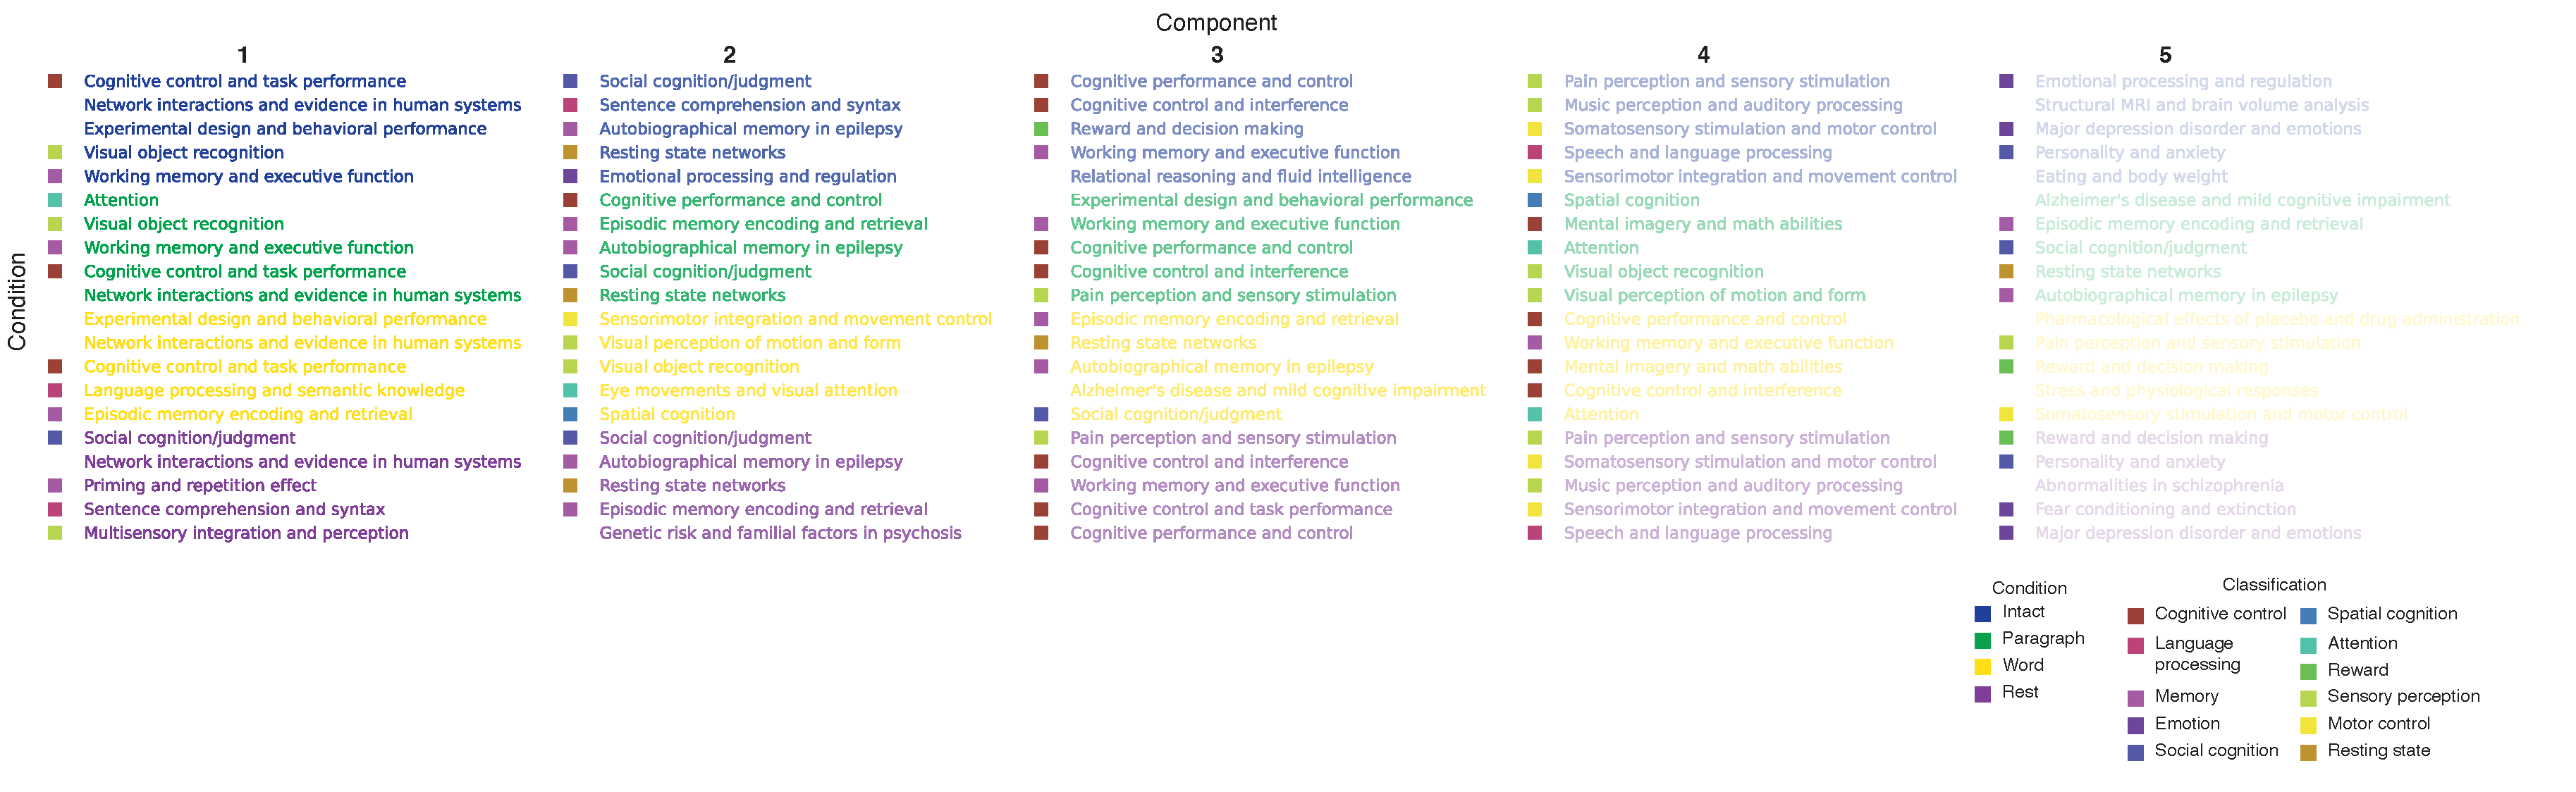
\includegraphics[width=\textwidth]{figs/top_terms_by_component}

\caption{\textbf{Top terms associated with the highest-weighted components by
condition, broken down by story segment.} Each group of five rows corresponds
to an experimental condition (denoted by color, as indicated in the legend in
the lower right), and the columns and shading correspond to the component
number (ranked by proportion of variance explained). The colored squares in
front of many of the topics denote manually identified cognitive labels
(Tab.~S1).}

\label{fig:top-terms}
\end{figure}

\begin{figure}
  \centering
  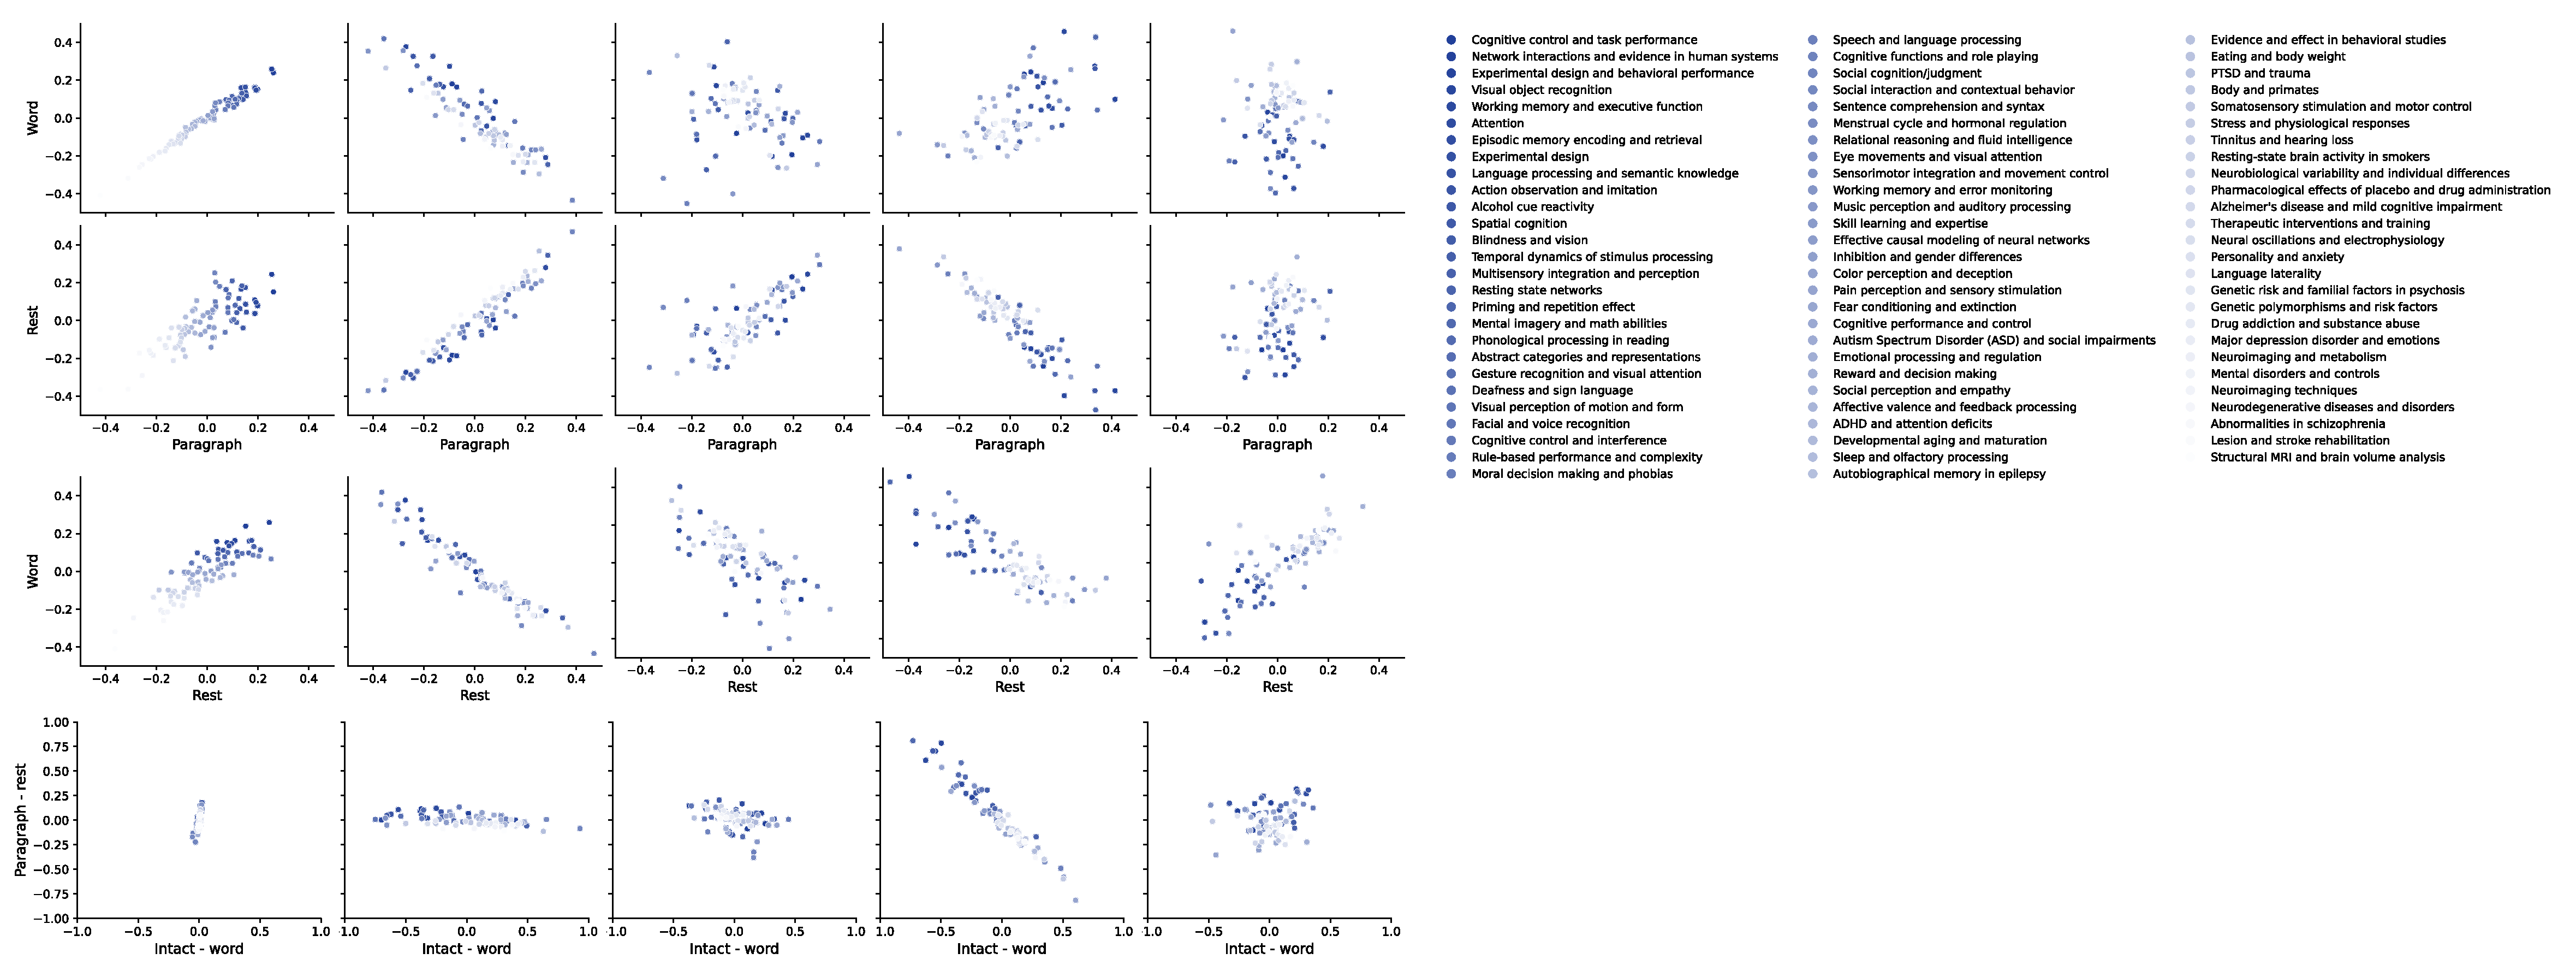
\includegraphics[width=\textwidth]{figs/topic_contrasts}

\caption{\textbf{Fill this in...}}

\label{fig:contrasts}

\end{figure}

\newpage
\renewcommand{\refname}{Supplemental references}
\bibliographystyle{apacite}
\bibliography{CDL-bibliography/cdl}

\end{document}


